\chapter{Конструкторский раздел}

\begin{figure}[h!]
	\begin{center}
		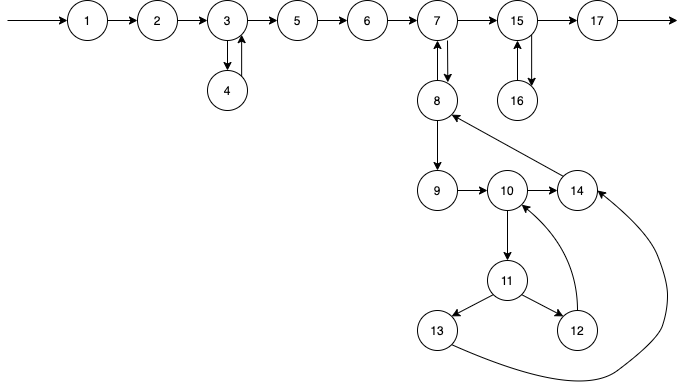
\includegraphics[scale=0.6]{assets/0.png}
	\end{center}
	\caption{Операционный граф}
\end{figure}

\begin{figure}[h!]
	\begin{center}
		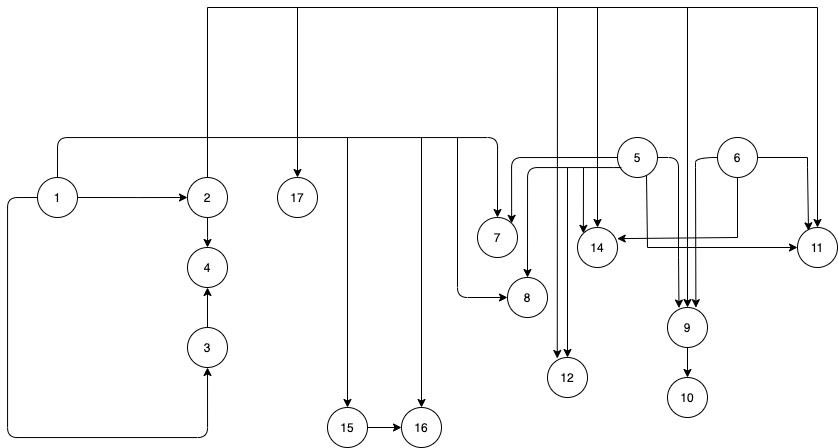
\includegraphics[scale=0.6]{assets/1.png}
	\end{center}
	\caption{Информационный граф}
\end{figure}


\begin{figure}[h!]
	\begin{center}
		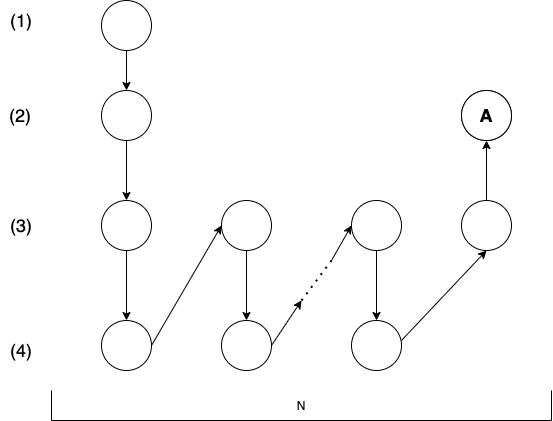
\includegraphics[scale=0.6]{assets/2.png}
	\end{center}
	\caption{Операционная история программы часть 1}
\end{figure}

\begin{figure}[h!]
	\begin{center}
		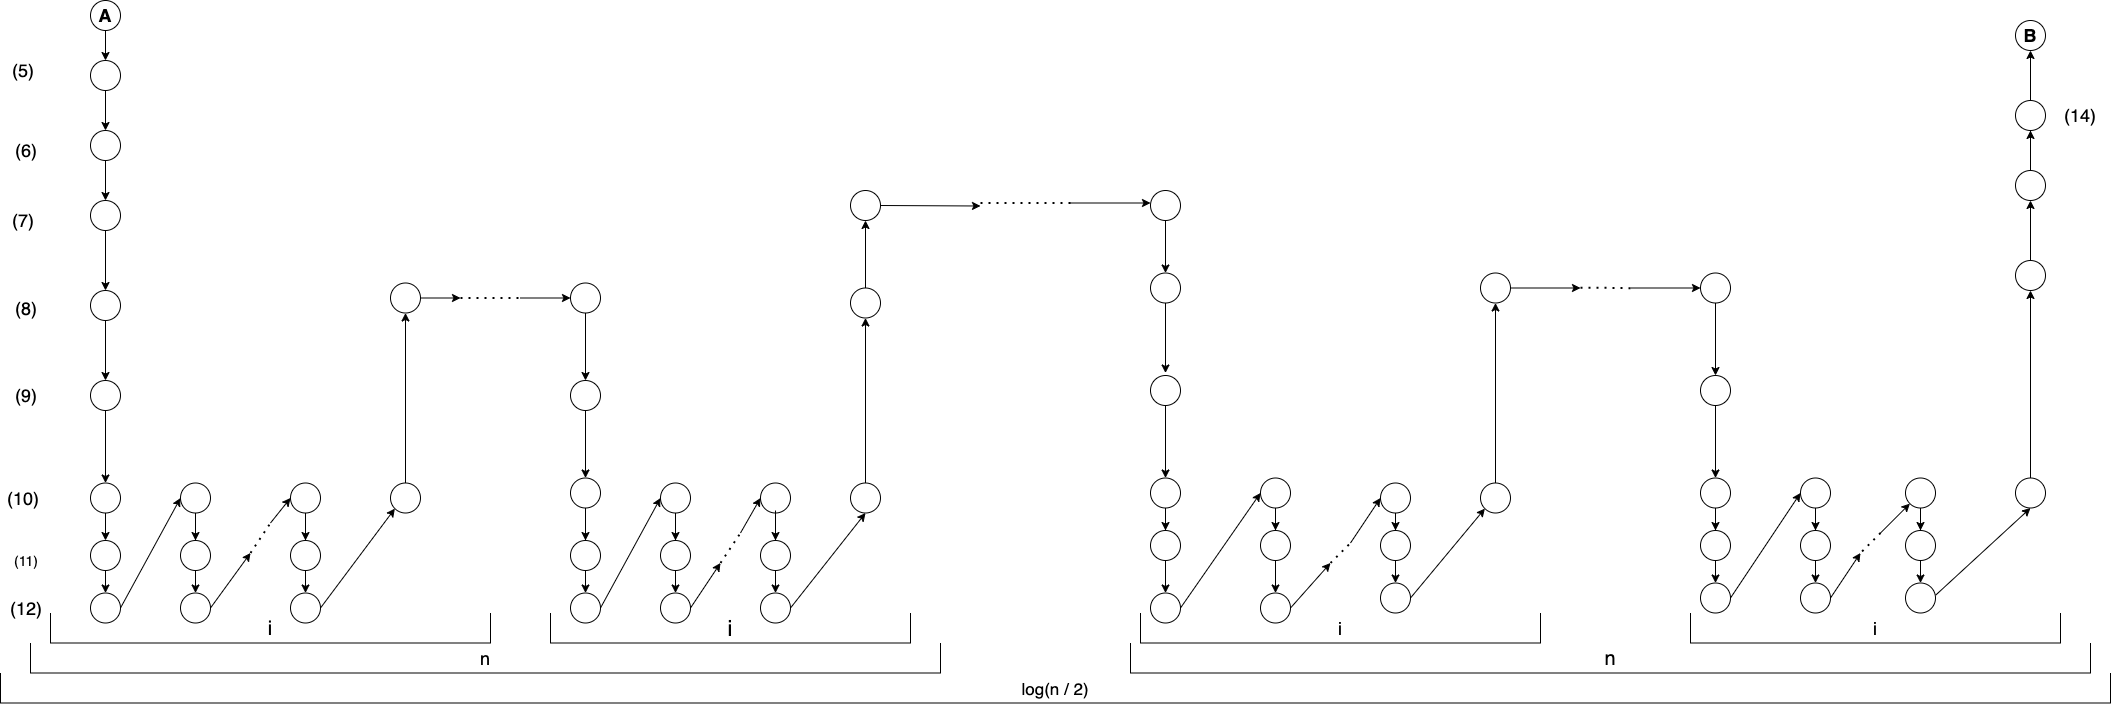
\includegraphics[scale=0.24]{assets/2_2.png}
	\end{center}
	\caption{Операционная история программы часть 2}
\end{figure}


\begin{figure}[h!]
	\begin{center}
		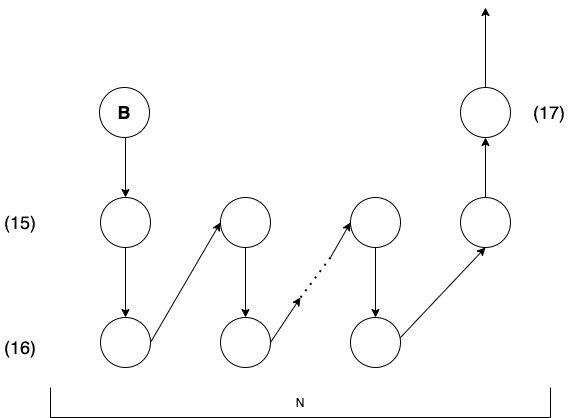
\includegraphics[scale=0.6]{assets/2_3.png}
	\end{center}
	\caption{Операционная история программы часть 3}
\end{figure}



\begin{figure}[h!]
	\begin{center}
		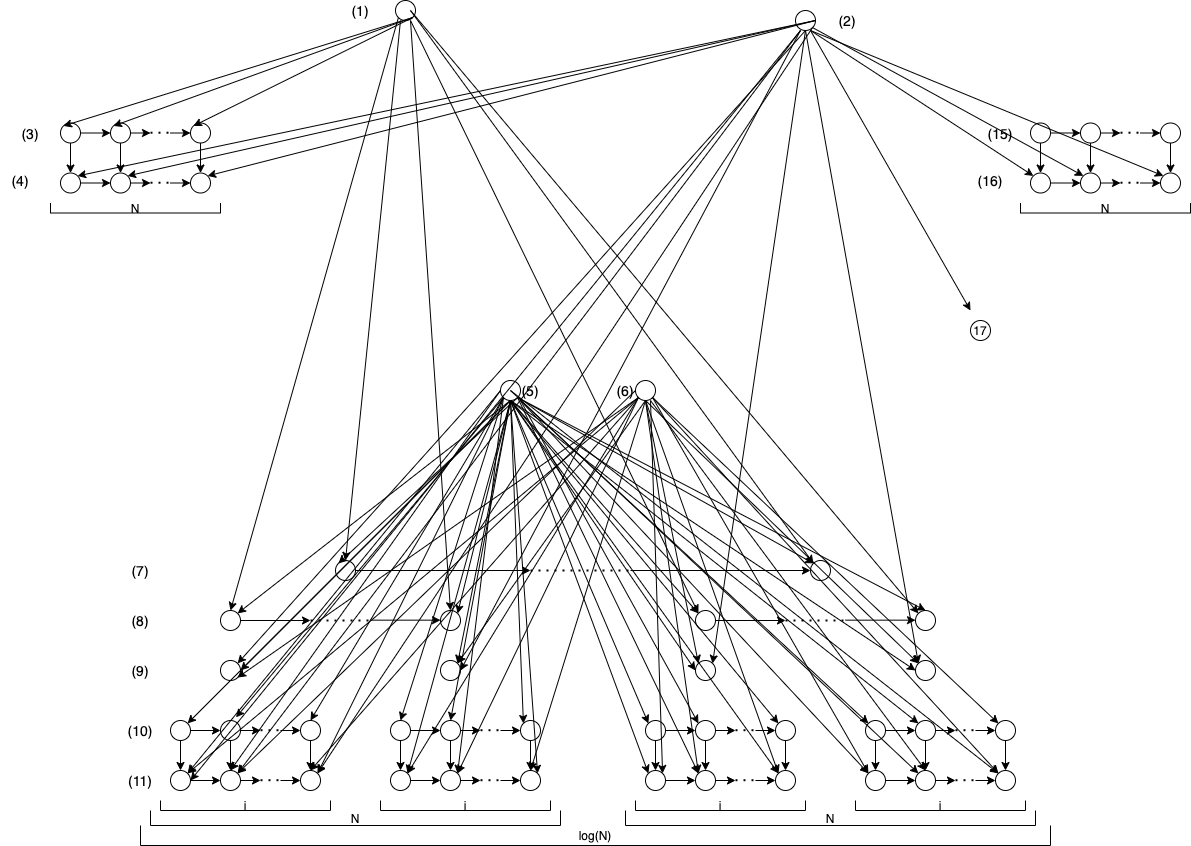
\includegraphics[scale=0.4]{assets/3.drawio.png}
	\end{center}
	\caption{Информационная история программы}
\end{figure}